\documentclass{article}
\usepackage{tikz, comment}
\usepackage{pifont}
\usepackage{fontspec, pgfplots}
\usetikzlibrary{arrows, decorations.markings, decorations.pathreplacing}
\begin{comment}
:Title: Not defined yet
:Tags: moment;pappus&#146;s theorem, theorem of pappus;perimeter;median of a trapezoid;arc length of a curve
:Prob: 0.5713;0.569;0.5668;0.5567;0.5517
:Author: Prof.Hu Ji-shan, HKUST
:Slug: No name yet

Description Here.........
\end{comment}
\begin{document}\centering 

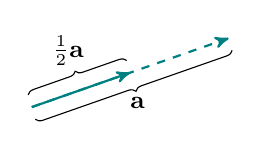
\begin{tikzpicture}[>=latex,xscale=.5*5, yscale=.5*5][font=\sf\small] 

\draw[dashed, teal, thick, ->, >=stealth'] (0, 0) -- (1, 0.35);
\draw [decoration={brace,raise=2, mirror},decorate, xshift=0.25, yshift=-1]
(0, 0) -- (1, 0.35)node[black, below, midway, pos=0.5, xshift=2, yshift=-3, scale=1]{$\bf a$}; %a

\draw[teal, thick, ->, >=stealth'] (0, 0) -- ({1/2}, {0.35/2});
\draw [decoration={brace,raise=2},decorate, xshift=-0.25, yshift=1] 
(0, 0) -- ({1/2}, {0.35/2})node[black, above, midway, pos=0.5, xshift=-4, yshift=3, scale=1]{$\frac{1}{2}\bf a$};

\end{tikzpicture}
\end{document}